\section{Context}
\label{sec:Context}


\subsection{Dataset}
\label{sec:dataset}
\begin{figure}
    \centering
    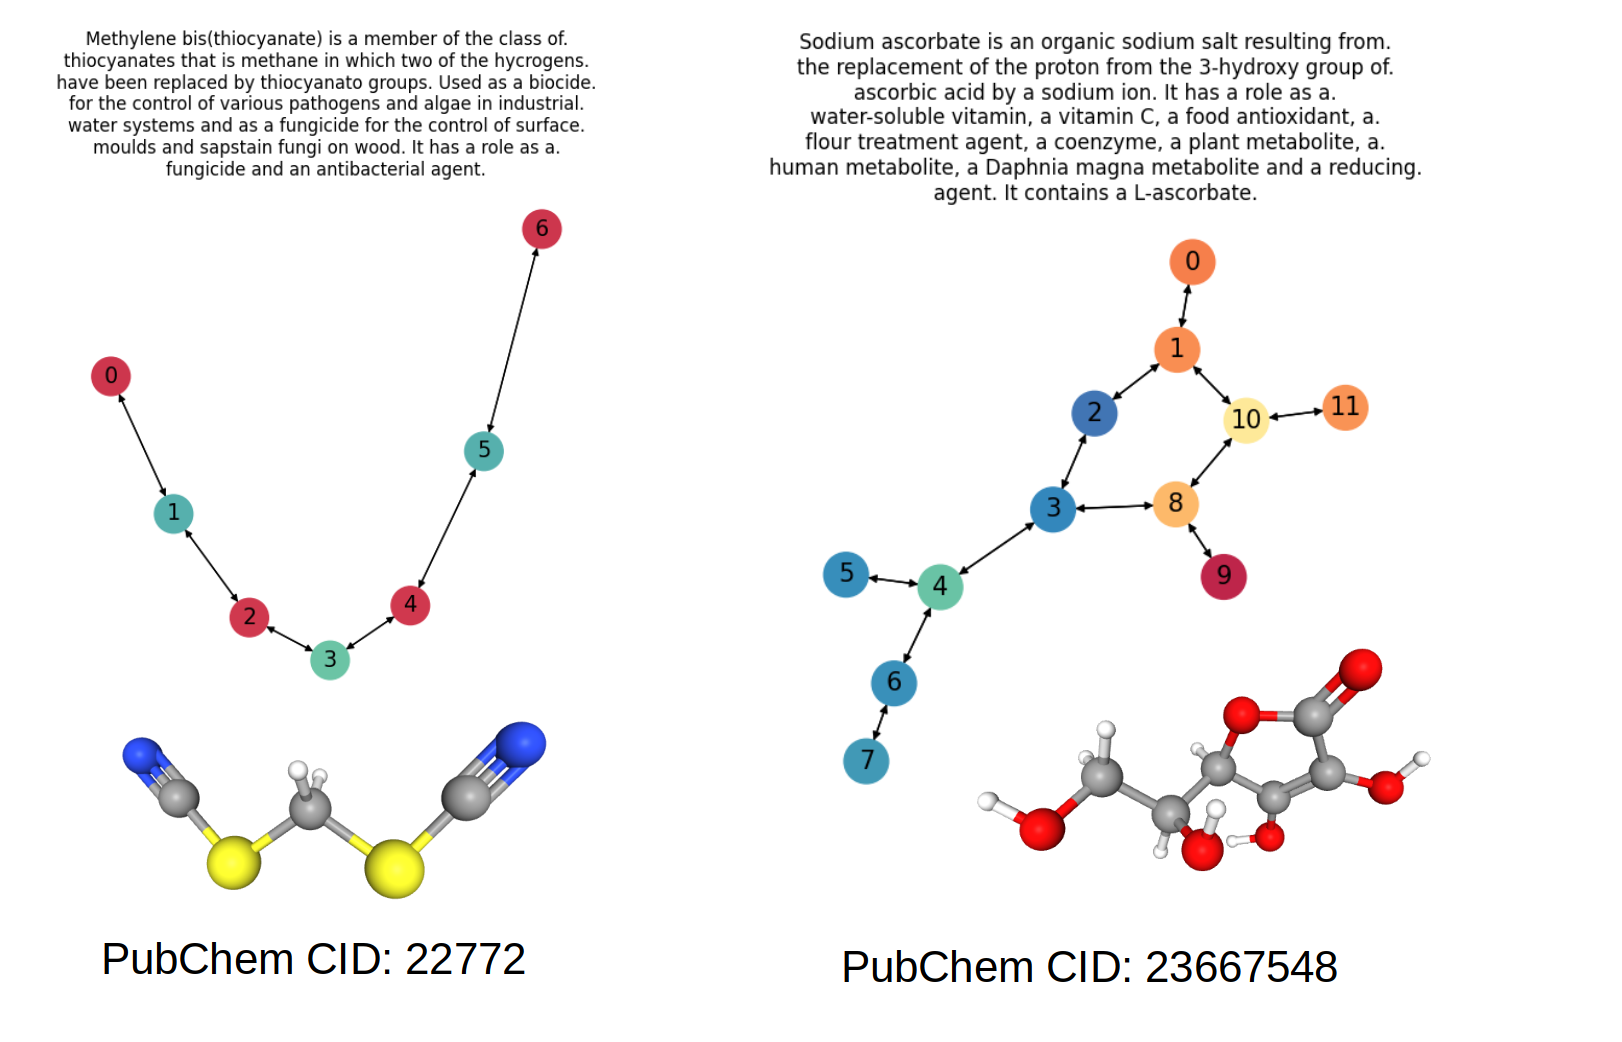
\includegraphics[width=1.\linewidth]{figures/molecule_visualizations.png}
    \caption{2 samples of molecules compounds paired with their description (matching correctly with their unique identifier on PubChem). These two examples show the difficulty of the task, both descriptions include the word Water being used in very different contexts. The Mol-2-Vec token ids (represented with colors in the graph) model more than atoms (molecule structures in their context neighborhood)}
    \label{fig:molecule_sample}
\end{figure}
The provided dataset is made of pairs of molecules and text descriptions. Text-2-Mol \cite{text2mol} came out with a dataset of 33 310 molecule paired with a textual description, made publicly available (which is always appreciated among the research community). Molecular structures (unitary structures slightly more generic than the atom level) have been isolated with their corresponding vector representations. Vector representation relies on Mol2Vec\cite{mol2vec} which is a machine learning algorithm to create vector representations of molecular substructures trained in an unsupervised manner over 19.9 millions of chemical compounds. In figure \ref{fig:original_pipeline}, this step corresponds to the graph features extractor step. Each node is paired with a vector of length 300 which naturally contains a lot of information about the nature of the molecular substructure (this feature representation is far more powerful than simply depicting a single atom for instance). In the Mol-2-Vec dictionary, there are 3137 tokens types (+1 unknown), each token id corresponds to a vector of dimension 300.
The provided dataset has been split into 80\% , 10\%, 10\% (train, validation, test - see table \ref{tab:dataset_stats}).

\begin{table}
    \centering
    \begin{tabular}{|c|ccc|}
    \hline
         Split &  Train &  Validation& Test\\ \hline  
         Split ratio &  80\% & 10 \% & 10\% \\ \hline  
         Graph/Text pairs&  26408&  3301& 3301\\ \hline  
         Groundtruth&  Yes&  Yes& Not public\\ \hline 
    \end{tabular}
    \caption{Dataset split}
    \label{tab:dataset_stats}
\end{table}

\subsection{State of the art}
\label{sec:sota}
In the following section, we'll briefly describe relevant work related to our topic (a more thorough study is available in Appendix \ref{sec:sota_long_version}).
CLIP \cite{CLIP} builds image representation embedded in the same vector space as textual representations and works with augmented pairs of image/text by batches of size 32000. 

Text-2-Mol \cite{text2mol} applies the same concept to molecules represented as graphs (rather than regular image grids) and uses graph convolutional networks (GCN \cite{kipfwellinggcn}) to extract meaningful information. Text-2-Mol uses tiny batches of size 32 compared to CLIP. Text-2-Mol fine tunes SciBERT (a transformer encoder \cite{scibert}) pretrained by masked language modeling on a corpus of 1 million of scientific articles. 

Molecule augmentations (atom masking, bounds deletion, subgraphs deletion) are proposed in Mol-CLR\cite{molCLR}, a contrastive learning approach applied to molecule graphs only (like SimCLR \cite{SIMCLR} or the recent DINO \cite{DINO} which work solely on images, but here transposed to molecules).